\graphicspath{{../images/ch5/}}	% Image directory


\chapter{Resistive pulse studies of cancer cell deformability}

	

	\section{Background \& Theory}
	      
		One of the most important applications in microfluidic technology today is the study of cell populations. The most important tool for studying cell properties is the flow cytometer, invented in 1965 by Fulwyler \cite{Fulwyler1965}, and is conceptually the follow up to Coulter counters which can be considered to be impedance cytometers. Flow cytometers are a mixture of many individual microfluidic elements combined in series, each with its own function. On the sensing side, flow cytometry makes use of measured scattering of laser light as well as detection of fluorescence signals. Dyes are specifically attached to certain types of antibodies, which then may interact with the cell membranes in the suspension. When the cells are pulsed by lasers in the laser light, it stimulates emission of specific dyes, which can be measured to determine which antibodies have interacted with the cell. This type of information is incredibly value in determining phenotypic and classification information for the cells. Furthermore, the information garnered from real-time cytometry information can be used to sort cells in real time, in a system known as fluorescence activated cell sorting system (FACS). Cell cytometry is the workhorse of modern day molecular and cellular biology studies, but suffers from the fact that it is a label-dependent method due to the introduction of the dyes. Such labels can adversely affect the the cells' viability that prevents them from being used in a post-interrogation analysis, even after being separated by a system like FACS. Additionally, flow cytometry requires the use of costly fluorescent reagents and skilled technicians that must be present to perform the measurement and to ensure proper calibration of the fluorescence signal \textit{via} the use of fluorescent beads \cite{Gosset2012} (DiCarlo PNAS).
	
		While flow cytometry focuses on the measurement of cells' interactions with specific antibodies, another dimension often not thought of is the cells' mechanical properties, such as their size, shape, deformability, and deformability dynamics \cite{Lin2017} (DiCarlo paper in Nature 2017). Since their discovery, we've known that a wide variety of cell sizes exist, but more recently scientists have focused on the difference in the mechanical stiffness of cells. Cell stiffness has been shown to vary from cell to cell, and even between various stages in cells' mitotic cycles. As a concrete example, cancer cells are known to be generally `squishier' than non-cancerous cells. For these reasons, developing a method of probing the mechanical stiffness of cells is highly desirable for cell characterization applications, and serve as a complementary cell phenotyping platform to deformability cytometry.
		
		In order to measure the stiffness of an object, it must be subjected to constrained forces and its response measured. Probably the most straight forward way of doing this is by directly applying a mechanical force on the cell, for example by using an atomic force microscopy (AFM) probe to directly press on the cells and measure the resultant recoil force felt by the AFM's cantilever, which is directly related to the Young's modulus of the cell. Other similar methods exist, and while they are very accurate and easily interpretable, they suffer from an excruciatingly slow throughput. For instance, using AFM for cell deformation measurement can take a few minutes per cell. For cell applications a high throughput is necessary, and therefore these applications are not feasible for discovering cell population statistics.
		
		Another method of measuring cell deformability is with microfluidics platforms. Cells passing quickly through narrow constrictions are subjected to large, anisotropic hydrodynamic forces, and these forces can induce a measurable particle deformation. The advantage of this type of method is its extremely large throughput; rather than spending several minutes per particle as in measurements conducted with AFM, thousands of cells per second can be measured in microfluidic platforms. Even within the narrow field of microfluidic-based deformability cytometry, there are multiple types of platforms. Probably the most conceptually simple is a standard microfluidic channel that tightly confines cells passing through it. Due to anisotropies in the hydrodynamic stresses and strains around the particle, it will deform even in a uniformly shaped channel.
		
		In traditional microfluidic methods of measuring cell deformability, direct imaging is used to determine the cell shape across different frames in the video, which corresponds to the hydrodynamic load it is under. However, for the high throughputs that are the reason why people use microfluidics, camera imaging must be performed very quickly. This requires the use of a high-speed camera used in conjunction with an optical microscope, usually shooting at a minimum of $\SI{10000}{fps}$. When combined with an optical microscope, such high-speed cameras are capable of capturing cell deformations with high spatial and temporal resolution, and are even capable of resolving the cells' deformation dynamics \cite{DiCarlo2017}. Currently high-speed camera imaging is by far the most popular method of capturing cell deformations, but it comes with two serious disadvantages. First, the camera itself adds a large cost to the apparatus, and will likely dwarf the price of any other component in the deformability cytometer. Second, imaging data is inherently highly multidimensional and computationally expensive to analyze. As a result, online analyses conducted during the run of the experiment are usually not possible at the flow rates that these experiments operate at. While the data can still be stored, processed, and analyzed later, offline analysis does not allow for real-time separation, one of the most highly desirable applications of this type of metrology.
		
		Instead of using camera imaging, one can instead imagine trying to employ resistive pulse (RP) to measure the deformability of particles. In terms of practicality, RP is far more computationally light than imaging data, as the following order of magnitude estimate shows. Passage through a deformability cytometry system may consist of $\sim100$ frames, each with a resolution of perhaps $100x50$ 8-bit grayscale valued pixels. As a result, the entire translocation is described by $\SI{500}{kB}$ worth of data. At a rate of $1000$ particles per second, this corresponds to a raw data throughput of $\SI{500}{MB/s}$ of data that must be analyzed. Finally, in a common image processing algorithm the number of computations performed on each pixel is probably greater than one; identifying the shape of an object in a frame certaintly consists of multiple image processing steps performed serially. Although this is just an estimate, it conveys the point that high-speed imaging is not amenable to online analysis, especially at the throughputs that are desired for these types of calculations. On the other hand, consider a resistive pulse analysis: under the same criteria described above, an RP data stream being sampled at $\SI{1}{MHz}$ will consist of a data throughput of only $\SI{1}{MB/s}$, a factor of $500$ decrease.
		
		While it is apparent that resistive pulse is computationally cheaper than imaging analysis, it is most important to demonstrate that deformability can actually be measured via RP sensing. In chapter 4 of this dissertation, we discussed the equations for the resistive pulse amplitudes of ellipsoidal objects. For cells that are spheroidal in their unloaded state, ellipsoids are reasonable geometries to expect for the deformation shape in the loaded state, at least as an approximation. If we consider a straight ion conducting channel with an ellipsoidal particle inside it, the aspect ratio and orientation of the particle greatly affects the ionic resistance of the system. Under the assumption that the particles take on ellipsoidal geometries, the shapes will be described as being prolate, oblate, or spherical with respect to the channel's axis. Oblate geometries correspond to a flattening along the channel's axis, and prolate geometries are an extension along the channel's axis. The difference in the measured resistive pulse amplitude of these particles is given by the following equation:
		
		\begin{equation} \label{eq:ellipsoiddI}
			\frac{\Delta I}{I_{p}}=f_{\parallel}\frac{v}{V},
		\end{equation}
		
		where $v$ and $V$ are the volume of the particle and channel, respectively, and $f_{\parallel}$ is a constant known as the `shape-factor', which depends on the aspect ratio of the ellipsoid. 
		
		\begin{figure}
			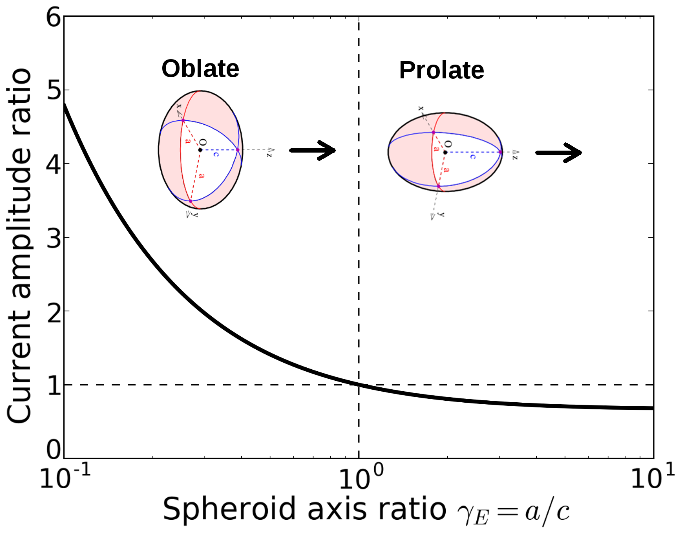
\includegraphics[width=0.5\textwidth]{dIellipsoid.png}
			\caption{\textbf{Resistive pulse amplitude $\Delta I/I_{p}$ for equal volume spheroidal objects relative to a sphere.} The polar axis of the particle is aligned with the channel's axis, so that oblate geometries correspond to motion along the channel axis. The values come from equation \ref{eq:ellipsoiddI} when the correct shape factor $f_{\parallel}$ is applied.}
		\end{figure}

		
		For spheres, $f_{\parallel}=1$, and for prolate and oblate spheroids, $f_{\parallel}<1$ and $f_{parallel}>1$, respectively. Figure \ref{fig:dIellipsoid} shows plots of the RP amplitude $\Delta I/I_{p}$ for ellipsoids of the same volume but different aspect ratios, relative to a sphere. The plot reveals that even for modest deformation, for instance a stretching ratio of $2/3$, a mildly oblate ellipsoid, the increase in $\Delta I/I$ is nearly $30\%$. Similarly, the current $\Delta I/I$ changes for prolate geometries, although to a lesser degree.

		
		


%%% Local Variables: ***
%%% mode: latex ***
%%% TeX-master: "thesis.tex" ***
%%% End: ***
